\documentclass[serif]{beamer}  % for 4:3 ratio
\usepackage[T1]{fontenc} 
\usepackage{hyperref}
\usepackage{latexsym,amsmath,xcolor,multicol,booktabs,calligra}
\usepackage{graphicx,pstricks,listings,stackengine}

\author{
    Giovanni Billo
    \and  
    Andrea Suklan
    \and  
    Carlos Velázquez Fernández
}
\title{Analysis of RL Algorithms for a Simulated Hill Climb Racing Agent}
\date{\small July 28, 2025}
\usepackage{UoWstyle}

% defs
\def\cmd#1{\texttt{\color{red}\footnotesize $\backslash$#1}}
\def\env#1{\texttt{\color{blue}\footnotesize #1}}
\definecolor{deepblue}{rgb}{0,0,0.5}
\definecolor{deepred}{RGB}{153,0,0}
\definecolor{deepgreen}{rgb}{0,0.5,0}
\definecolor{halfgray}{gray}{0.55}

\lstset{
    basicstyle=\ttfamily\tiny,
    keywordstyle=\bfseries\color{deepgreen},
    emphstyle=\ttfamily\color{deepred},    % Custom highlighting style
    stringstyle=\color{deepblue},
    numbers=left,
    numberstyle=\tiny\color{halfgray},
    rulesepcolor=\color{red!20!green!20!blue!20},
    frame=shadowbox,
}


\begin{document}


\begin{frame}
    \vfill
    \begin{center}
        
\includegraphics[keepaspectratio, scale=0.15]{images/logo.jpg}
        
        \vspace{1cm}
        
        \begin{beamercolorbox}[wd=\textwidth,center,rounded=true]{title}
            {\textbf{Analysis of RL Algorithms for \\ a Simulated Hill Climb Racing Agent}}
        \end{beamercolorbox}
        
        \vspace{1cm}
        
        {July 28, 2025}
    \end{center}
    \vfill
\end{frame} 

\begin{frame}    
\tableofcontents[sectionstyle=show,
subsectionstyle=show/shaded/hide,
subsubsectionstyle=show/shaded/hide]
\end{frame}



\section{Problem Definition}

    \begin{frame}{Markov Decision Process}

    A MDP is a \textbf{stochastic model for sequential decision making} defined by a tuple: $$(\mathcal{S}, \mathcal{A}, \mathcal{P}, \mathcal{R}, \gamma)$$.
        
    \end{frame}

    \begin{frame}{State Space ($\mathcal{S}$)}
        \begin{figure}
            \centering
            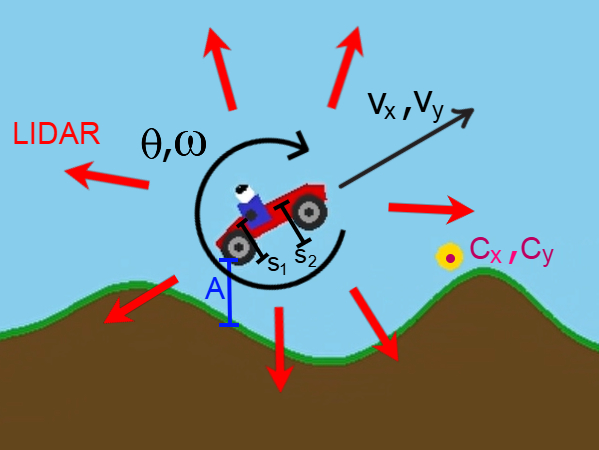
\includegraphics[width=0.8\linewidth]{images/state_space.jpg}
        \end{figure}
    \end{frame}

    \begin{frame}{Action Space ($\mathcal{A}$)}
        \begin{figure}
            \centering
            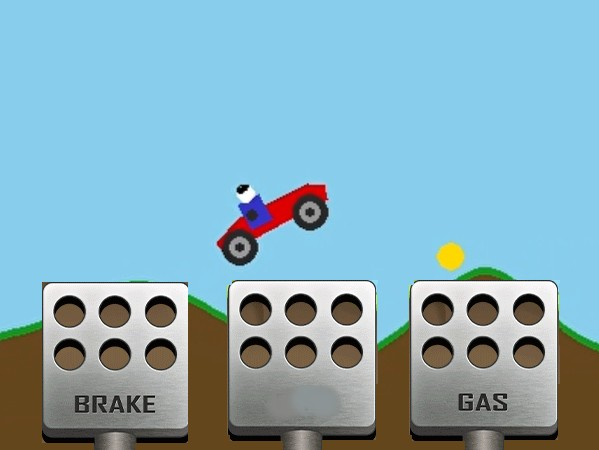
\includegraphics[width=0.8\linewidth]{images/action_space.jpg}
        \end{figure}
    \end{frame}

    \begin{frame}{Transition Dynamics ($\mathcal{P}$)}
        
    \end{frame}

    \begin{frame}{Reward Function ($\mathcal{R}$)}
        \centering
        \renewcommand{\arraystretch}{1.5}
        \begin{tabular}{l r}
            \toprule
            \textbf{Event} & \textbf{Value} \\
            \midrule
            Forward Progress (per meter) & +5.0 \\
            Coin Collection & +20.0 \\
            Air Time (per second) & +5.0 \\
            Time Penalty (per step) & -0.1 \\
            Crash (Episode End) & -50.0 \\
            \bottomrule
        \end{tabular}
    \end{frame}

    \begin{frame}{Discount Factor ($\gamma$)}
        
    \end{frame}

    \begin{frame}{policy ($\pi$)}
        
    \end{frame}

    \begin{frame}{Problem Classification}
        \begin{figure}
            \centering
            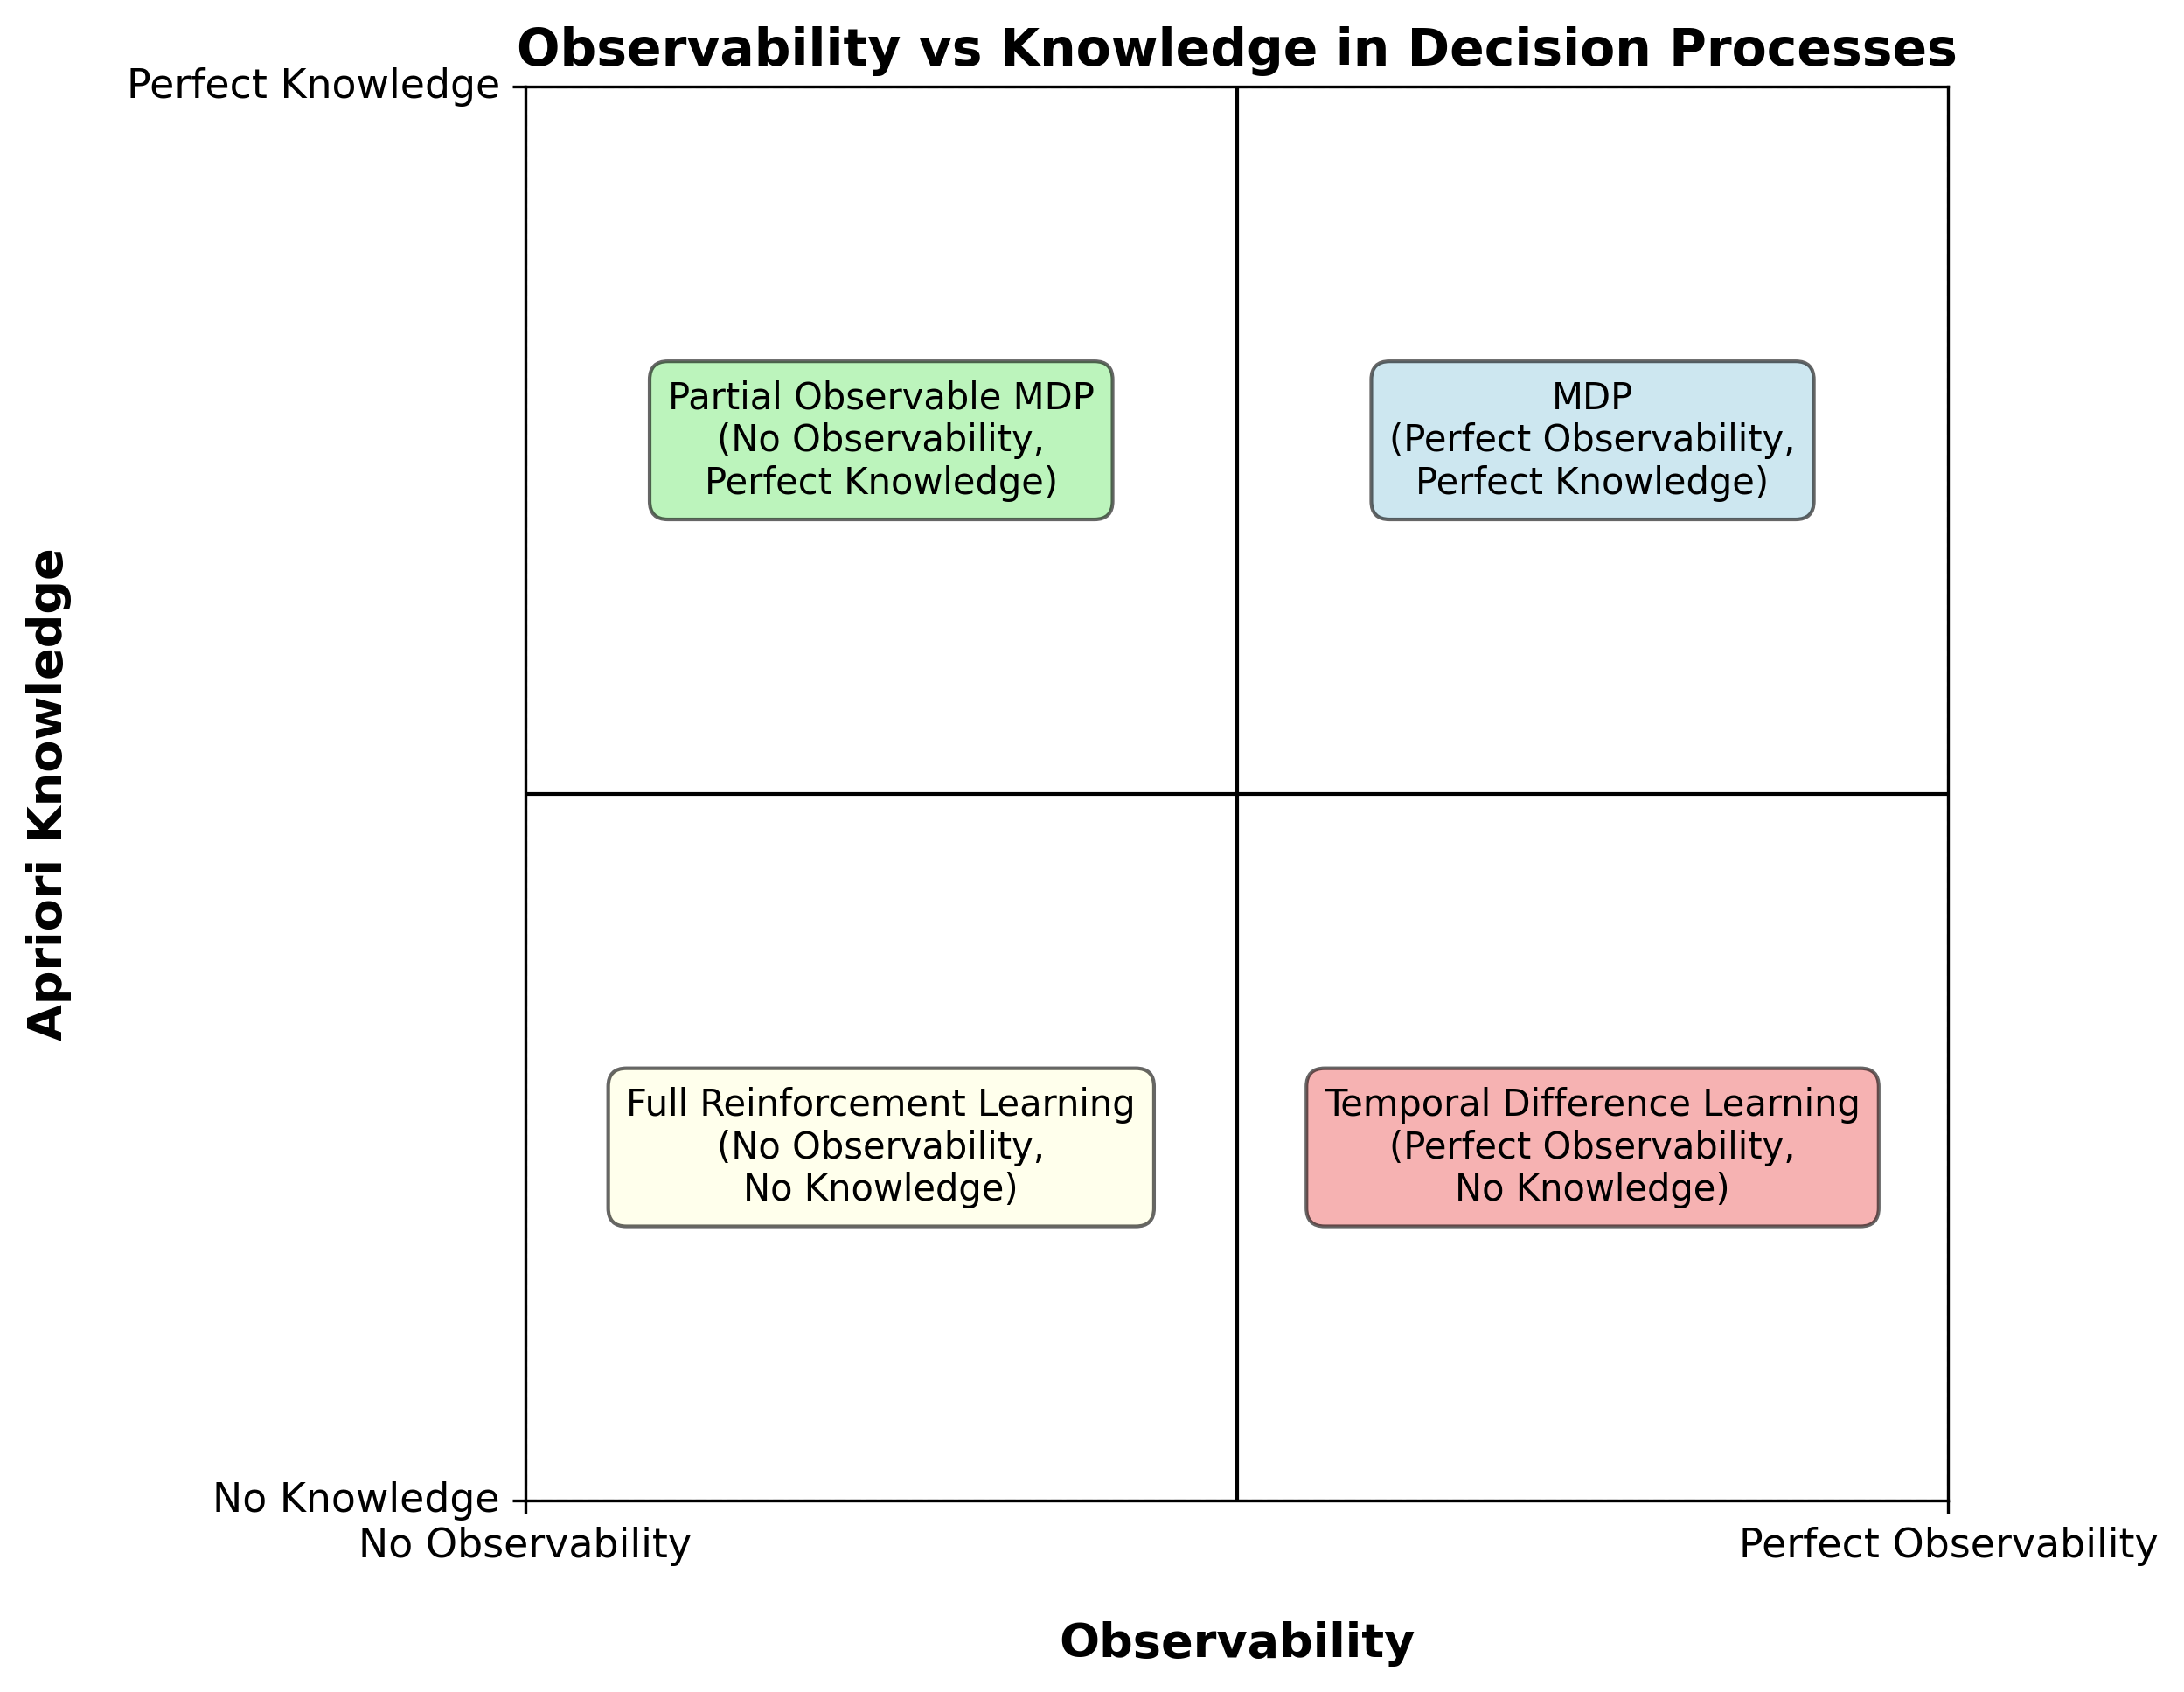
\includegraphics[width=0.8\linewidth]{images/knowledge_vs_observability.png}
        \end{figure}
    \end{frame}


\section{Deep Q-Network}


\begin{frame}{Characteristics of DQN}

    DQN combines the principles of \textbf{deep neural networks} with \textbf{Q-learning}.
    \vspace{1cm}
    \begin{itemize}
        \item \textbf{Off-policy:} learning from actions taken by different policies.
        \vspace{0.5cm}
        \item \textbf{Offline:} it collects a batch of experiences.
    \end{itemize}
\end{frame}

\begin{frame}{DQN Training}
    \begin{figure}
        \centering
        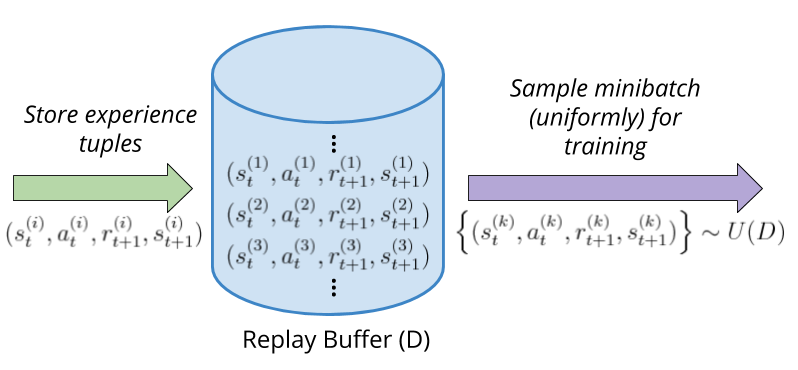
\includegraphics[width=0.8\linewidth]{images/experience_replay_buffer.png}
    \end{figure}
    \[L(\theta) = \left( \underbrace{r + \gamma \max_{a'} Q(s', a'; \theta)}_{\text{Target}} - \underbrace{Q(s, a; \theta)}_{\text{Prediction}} \right)^2\]
\end{frame}

\begin{frame}{DQN Algorithm}
    \begin{figure}
        \centering
        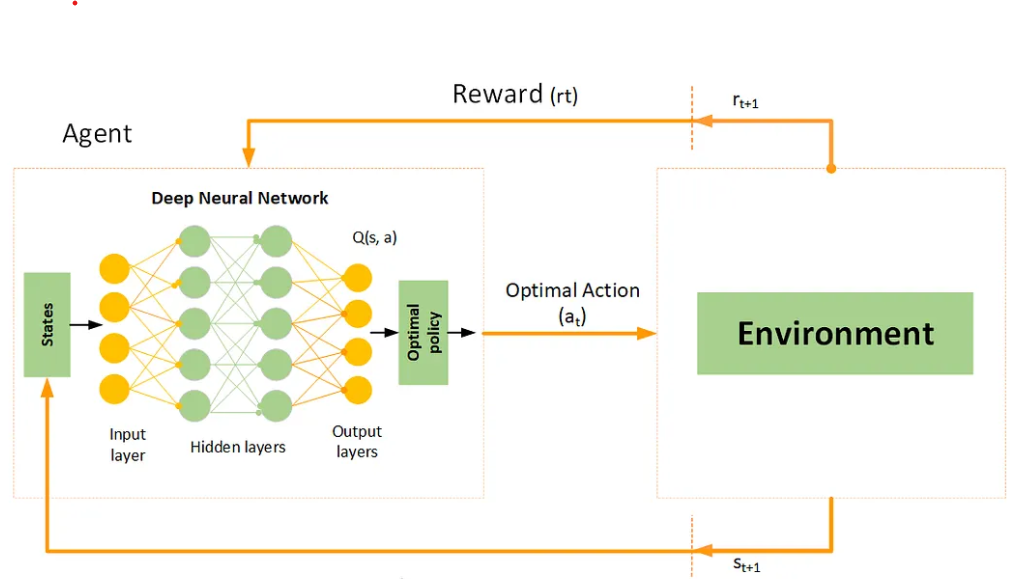
\includegraphics[width=\linewidth]{images/DQN_diagram.png}
    \end{figure}
\end{frame}


\section{Expected SARSA}

\begin{frame}{Exprected SARSA Algorithm}
    \begin{figure}
        \centering
        %\includegraphics[width=\linewidth]{images/ESARSA_diagram.png}
    \end{figure}
\end{frame}


\section{Proximal Policy Optimization}

\begin{frame}{PPO Algorithm}
    \begin{figure}
        \centering
        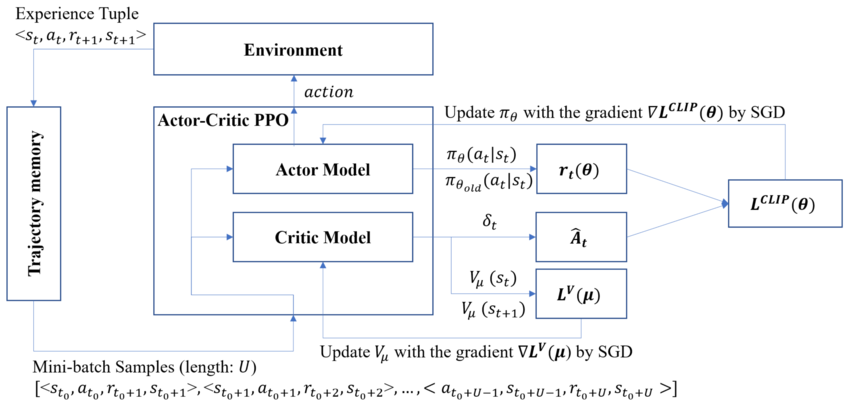
\includegraphics[width=\linewidth]{images/PPO_diagram.png}
    \end{figure}
\end{frame}


\section{Results}

\begin{frame}
\centering
{\Huge Thank you!}
\end{frame}

\bibliography{ref}
\bibliographystyle{plain}

\end{document}
